\section{Maxwell Evidence and the Limits of Structural Repair}
\subsection{Physical model and independent reference}
The finite-object computations use three-component Maxwell DDA with six transverse illuminations and two transverse receiver components. Material coordinates are real, including both parts of complex contrast, and orthonormalized in the volume-weighted material metric. The DDA injection retains $a'(\chi)E^{\rm tot}$ for the contrast-dependent polarizability $a$, rather than treating polarizability as contrast. The supplement gives the exact dyadic, self-term convention, material gauge, and real adjoint.

All principal calculations use FP64. Algebraic checks compare block elimination with direct Galerkin endpoints, their material steps, and the complete directional gain. Rank deficiency, complex phase and permutation changes, singular common cores, and CPU/CUDA consistency are included. Implementation consistency and continuum fidelity are checked separately.

A homogeneous sphere of radius 0.35, wavenumber 2, and contrast $1+0.05i$ provides an independent vector-Mie reference. At the finest $32^3$ grid the aggregate complex far-field error is 0.252\% and the uniform real-contrast derivative error is 0.731\%. Grid errors are nonmonotone; this validates the stated sphere response and uniform perturbation, not every voxel Jacobian direction. The coarse high-contrast sphere retains its 21.40\% independent discrepancy.

\subsection{Direct radiation can miss retained feedback}
Three constructed two-column current banks on $5^3$, $6^3$, and $7^3$ free-space grids have direct receiver norms below $1.7\times10^{-16}$. Their feedback-dressed norms are 0.0672, 0.0720, and 0.0888; their material derivative discrepancies are respectively 3.56\%, 3.98\%, and 5.22\% of the full Jacobian norm. A seeded material tangent generates the candidate currents, which are projected outside the receiver-row and retained-current spaces. These discrete witnesses isolate the additional route carried by retained currents. They establish existence, rather than its frequency among arbitrary current directions.

\begin{figure*}[tbp]\centering
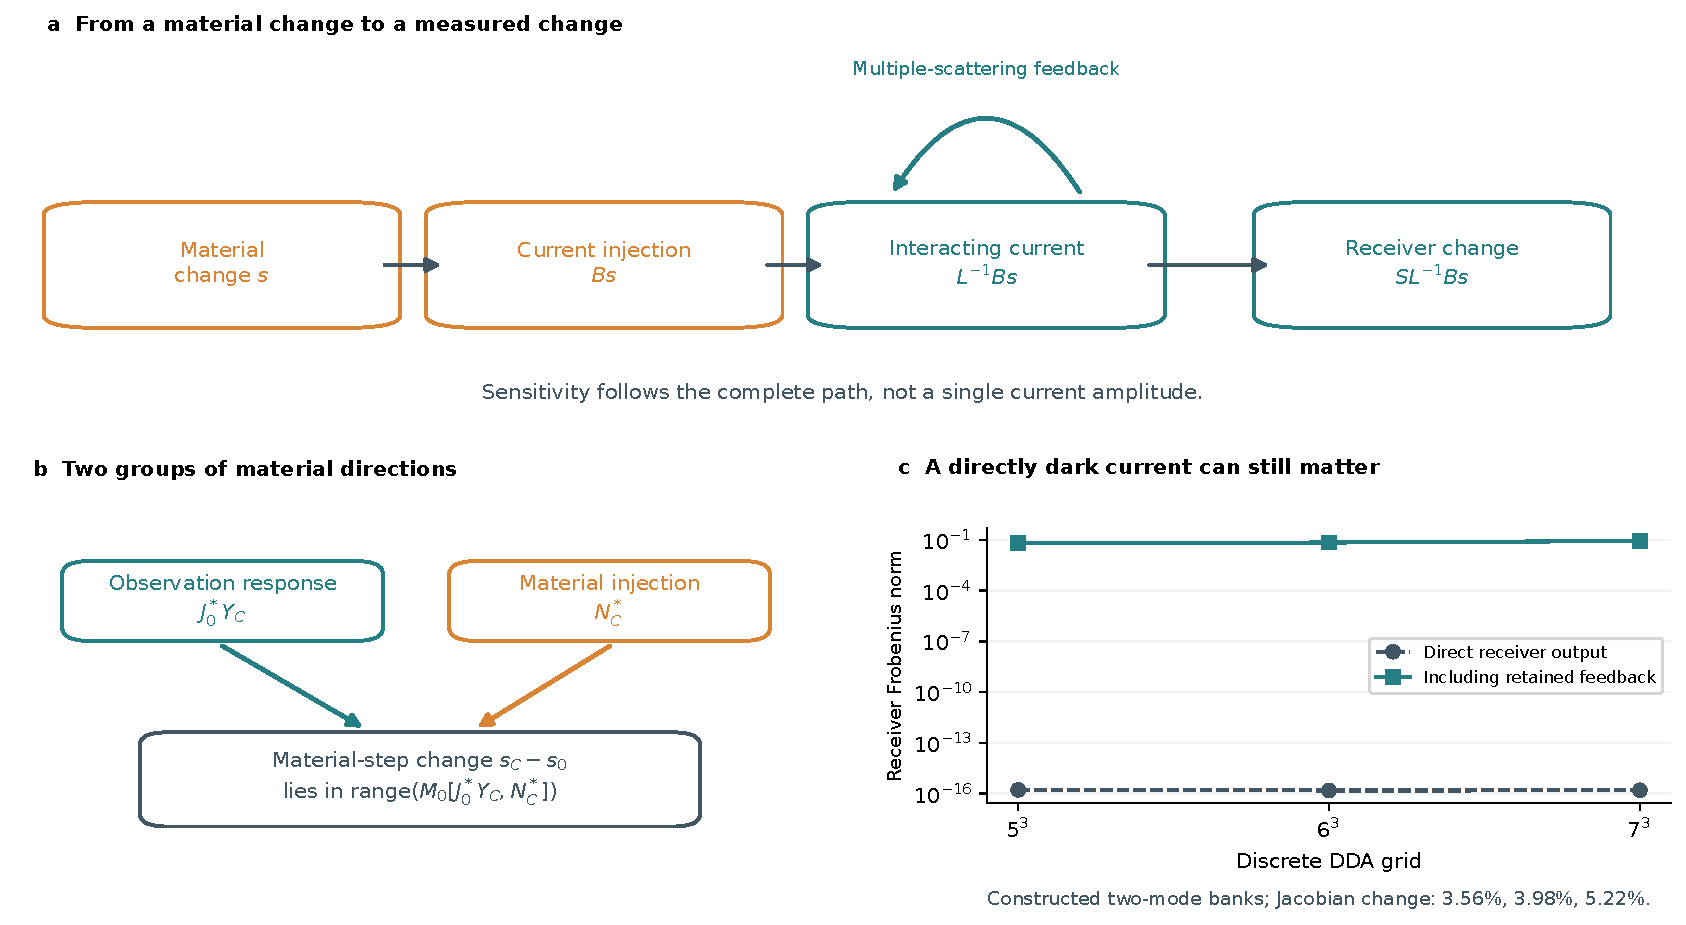
\includegraphics[width=.91\textwidth]{figures/material_paths.pdf}
\caption{A material perturbation enters the current equation and returns to the receivers through the interacting response. The numerical panel compares direct and retained-feedback outputs of constructed free-space Maxwell currents. The small direct output is at FP64 roundoff; the feedback response is resolved within the discrete model.}
\end{figure*}

\subsection{Closure, optimization, and cost give different answers}
Paired material repair reduces full-quadratic error more than its specified direct current enlargement in all 72 smooth and all 36 sharp frozen-state comparisons. Equal-real-rank material Krylov correction is better than paired repair in every one of those comparisons. Thus exact step-change support does not identify the best equal-rank correction for the complete objective.

Five normalized closure checks miss their original tolerance, with absolute $H$-distance $1.06\times10^{-15}$--$3.43\times10^{-14}$. Their Schur condition numbers are 1.00020--1.00093. The precision traces support cancellation and small-denominator amplification, rather than ill-conditioned Schur inversion or established underflow. All five failed checks remain in the record.

The paid paired warm-start route costs 1.416 times matched ordinary PCG, and increases full-wave RHS from 66 to 342. A separate current-derived preconditioning use obtains eight-use cost ratios 0.773--0.877 across six objects when the history is already paid. Charging dedicated history acquisition makes all six ratios exceed one; cached Ritz recycling wins on two objects. These results distinguish physical structure from an economical way to acquire it.

The four sharp-target reconstructions also retain substantial relative material errors, 0.755, 0.750, 0.560, and 0.906. They constrain claims about interface recovery for that acquisition. The conditional exchanges below reuse frozen states and do not create new nonlinear reconstruction evidence.
